\section{Modello di Ising 1D}

Il modello di Ising 1D è uno dei pochi modelli della meccanica statistica che presenta una soluzione esatta.
Il reticolo che prendiamo in considerazione in questo caso è lineare, tale per cui ogni sito reticolare presenta 
solo due primi vicini. Lavorando con condizioni periodiche al contorno, l'N-esimo spin diventa un vicino del 
primo ed il sistema si chiude ad anello, come è possibile apprezzare in Figura \ref{fig: Ising1D_pbc}.

\begin{figure}[h!]
    \centering
    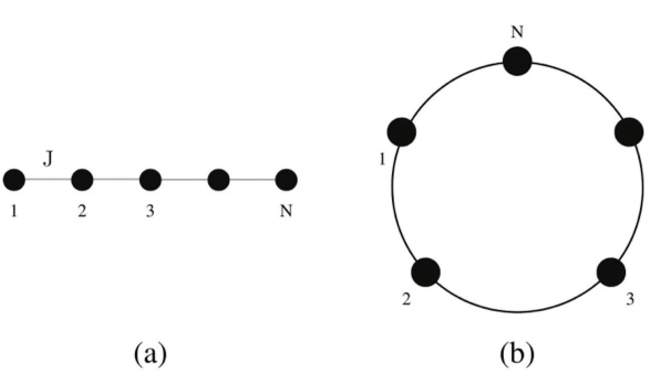
\includegraphics[width=0.7\textwidth]{Immagini/Ising1D_pbc.png}
    \caption{L'immagine (a) è un esempio di modello di Ising 1D senza pbc, mentre in (b) si può apprezzare 
    come la catena si chiuda su se stessa nel caso di condizioni periodiche al contorno. }
    \label{fig: Ising1D_pbc}
\end{figure}

Sebbene il modello di Ising 1D ammetta soluzione esatta, è istruttivo lavorare inizialmente con una teoria di campo 
medio, in cui il termine d'interazione presente nell'Hamiltoniana viene sostituito da un termine efficace (di campo 
medio appunto), andando a trascurare le fluttuazioni degli spin.





\subsection{Teoria di campo medio}

Il punto di partenza di una teoria di campo medio è la semplificazione del temine d'interazione presente nell'Hamiltoniana. Nel  
caso del modello di Ising mono-dimensionale l'interazione fra spin primi vicini può essere riscritta come

\begin{equation}
    \sigma_i \sigma_j\,=\,\left(\sigma_i\,-\,m\,+\,m\right)\left(\sigma_j\,-\,m\,+\,m\right)\,=\,-m^2\,+\,m\sigma_i\,+\,m\sigma_j\,+\,\left(\sigma_i\,-\,m\right)\left(\sigma_j\,-\,m\right),
    \label{eq: int_mf}
\end{equation}

dove l'ultimo termine della somma misura le fluttuazioni fra spin. L'approssimazione di campo medio consiste nel trascurare 
completamente l'ultimo termine, in modo tale che tutti gli spin risultino essere disaccoppiati fra loro e risulti più immediato il 
calcolo della funzione di partizione. L'Hamiltoniana di campo medio risulta quindi 

\begin{equation}
    H_{MF}\,=\,-\frac{J}{2} \sum_{\left<i,j\right>} \left[-m^2\,+\,m\left(\sigma_i\,+\,\sigma_j\right)\right]\,-\,h\sum_{i}\sigma_i,
    \label{eq: ham_mf}
\end{equation}

da cui è immediato il calcolo della funzione di partizione 

\begin{equation}
    Q_{MF}\,=\,\sum_{\left\{\sigma\right\}} e^{-\beta H_{MF}}\,=\,\exp{\left(-\frac{\beta J m^2 N n_{nn}}{2}\right)} \left\{2 \cosh{\left[\beta \left(J n_{nn} m\,+\,h\right)\right]}\right\}^N.
    \label{eq: part_MF_Ising1D}
\end{equation}

Nella relazione precedente la quantità $n_{nn}$ è il numero il numero di coordinazione del reticolo, ossia il numero di primi vicini per la 
geometria presa in considerazione. L'energia libera per particella è data da 

\begin{equation}
    \frac{F}{N}\,=\,-\frac{k_B T}{N} \ln{\left(Q_{MF}\right)}\,=\,\frac{JM^2n_{nn}}{2}\,-\,\frac{1}{\beta}\ln{\left\{2 \cosh{\left[\beta\left(h\,+\,Jn_{nn}m\right)\right]}\right\}}
    \label{eq: freeE_MF_Ising1D}
\end{equation}

da cui è possibile ricavare tutta la termodinamica del sistema.



\subsubsection{Magnetizzazione}

La magnetizzazione si ricava a partire dall'energia libera per spin mediante una derivata rispetto al campo magnetico $h$. 
La relazione che si ottiene è nota come \textit{equazione di Bragg-Williams}, che può essere espressa nella forma 

\begin{equation}
    \tanh^{-1}{\left(m\right)}\,=\,\frac{h\,+\,n_{nn}Jm}{k_B T}
    \label{eq: BW_equation}
\end{equation}

Nel caso in cui il campo magnetico è identicamente nullo, è necessario distinguere due casistiche in base alla temperatura del sistema. 
In primo luogo è necessario introdurre la temperatura critica 

\begin{equation}
    T_c\,=\,\frac{n_{nn}J}{k_B},
    \label{eq: tc_Ising1D_MF}
\end{equation}

che consente di riscrivere il secondo membro dell'equazione di Bragg-Williams in funzione del rapporto fra $T_c$ e la temperatura 
a cui il sistema si trova. Così facendo risulta evidente che quando $T\,>\,T_c$ l'unica soluzione possibile dell'equazione 
\eqref{eq: BW_equation} è $m\,=\,0$, ossia mancanza di magnetizzazione finita. Nel caso opposto, ossia con $T\,<\,T_c$, si hanno 
tre possibili valori di $m$, ossia $0,\,\pm m_0$, con $m_0$ quantità finita. L'energia libera consente di identificare quale 
sia la soluzione fisica, poichè come è possibile osservare in Figura \ref{fig: FE_Ising1D_MF} quando la temperatura scende al 
di sotto di quella critica $F$ passa da un regime in cui è presente un solo minimo in $m\,=\,0$ ad un regime con due minimi 
equivalenti in $m\,=\,\pm m_0\,\neq\,0$. 

\begin{figure}[h!]
    \centering
    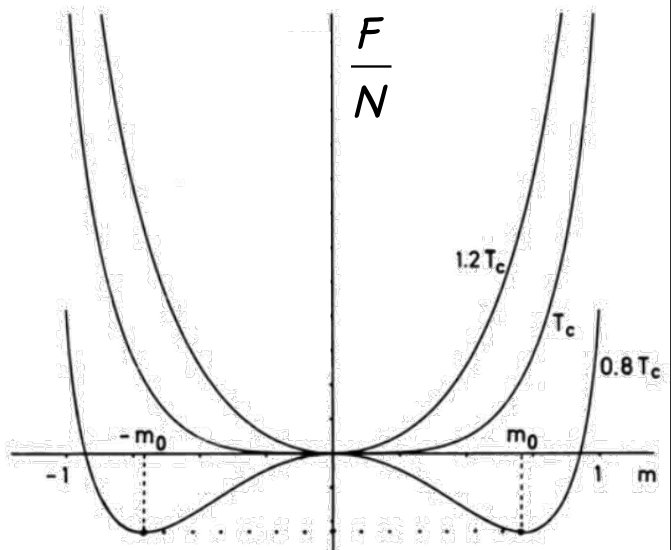
\includegraphics[width=0.7\textwidth]{Immagini/FE_Ising1D_MF.png}
    \caption{ Energia libera per particella al variare della temperatura del sistema. Quando la temperatura è maggiore o uguale 
    di quella critica è presente un solo minimo in $m\,=\,0$, mentre al di sotto sono presenti due minimi globali equivalenti e 
    simmetrici rispetto ad $m\,=\,0$, che è un massimo locale. Immagine da \cite{galliFSA}.}
    \label{fig: FE_Ising1D_MF}
\end{figure}

Questi due valori d'equilibrio della magnetizzazione sono perfettamente simmetrici in assenza di campo magnetico: una 
rottura spontanea della simmetria per inversione di spin è necessaria per far si che il sistema realizzi uno dei due stati di 
minimo globale dell'energia libera. 

Nel caso di campo magnetico esterno diverso da zero non si osserva più la simmetria caratteristica del caso con $h\,=\,0$ e l'
allineamento fra spin concorde con il verso di $h$ risulta essere energeticamente favorito.



\subsubsection{Esponenti critici}

E' possibile caratterizzare il comportamento di un certo sistema nell'intorno del punto critico in termini di leggi di potenza 
che presentano un set di esponenti critici. La seguente analisi è rivolta a 

\begin{table}[h!]
    \centering
    \begin{tabular}{|>{\centering\arraybackslash}p{2cm}|>{\centering\arraybackslash}p{11cm}|}
    \hline
    \textbf{Esponente} & \textbf{Significato fisico} \\ 
    \hline
    $\alpha$ & Descrive l'andamento del calore specifico al punto critico \\ 
    \hline
    $\beta$ & Descrive l'andamento del parametro d'ordine al punto critico \\ 
    \hline
    $\gamma$ & Descrive l'andamento della suscettività al punto critico \\ 
    \hline
    $\delta$ & E' legato all'equazione di stato alla temperatura critica \\ 
    \hline
    \end{tabular}
    \caption{Esponenti critici e relativo significato}
\end{table}

Procediamo ora al calcolo degli esponenti critici $\beta$ e $\delta$ per il modello di Ising mono-dimensionale. L'equazione di Bragg-Williams 
è uno strumento importante per il calcolo di $\beta$, poichè per $T\,\to\,T^-_c$ la magnetizzazione è molto minore di uno ed è possibile 
espandere in serie la tangente iperbolica tralasciando i termini di ordine superiore al terzo 

\begin{equation}
    m\,=\,\tanh{\left(m\frac{T_c}{T}\right)}\,\simeq\,m\frac{T_c}{T}\,-\,\frac{m^3}{3}\left(\frac{T_c}{T}\right)^3
    \label{eq: beta_fp_Ising1D_MF}
\end{equation}

in modo tale che, in seguito ad posto ad uno il fattore moltiplicativo del termine di grado 3, è possibile ricavare la 
magnetizzazione in funzione della differenza fra la temperatura critica e quella a cui si trova il sistema. Dato che 

\begin{equation}
    m\,\simeq\,\sqrt{3\left(\frac{T_c\,-\,T}{T_c}\right)}, 
    \label{eq: beta_sp_Ising1D_MF}
\end{equation}

l'esponente critico $\beta$ sarà pari ad un mezzo. Il calcolo di $\delta$ fa nuovamente uso dell'equazione di Bragg-Williams, che 
a temperature confrontabili con quella critica e per piccoli valori del campo magnetico, può essere espressa come 

\begin{equation}
    m\,=\,\tanh{\left(\frac{h}{k_BT}\,+\,m\frac{T_c}{T}\right)}\,\simeq\,\frac{h}{k_B T}\,+\,m\frac{T_c}{T}\,-\,\frac{1}{3}\left(\frac{h}{k_B T}\,+\,m\frac{T_c}{T}\right)^3
    \label{eq: delta_fp_Ising1D_MF}
\end{equation}

che porta all'equazione di stato approssimata 

\begin{equation}
    \frac{h}{k_B T}\,=\,m\frac{T\,-\,T_c}{T}\,+\,frac{m^3}{3}.
    \label{eq: beta_sp_Ising1D_MF}
\end{equation}

Considerando l'isoterma critica, il primo termine della somma a secondo membro scompare in modo tale che magnetizzazione e 
campo magnetico siano legati come 

\begin{equation}
    m\,\simeq\,\left(\frac{3h}{k_B T_c}\right)^{\frac{1}{3}},
    \label{eq: beta_tp_Ising1D_MF}
\end{equation}

che di conseguenza consente di identificare come $\delta\,=\,3$.





\subsection{Soluzione esatta}

Considerare un sistema con condizioni periodiche al contorno, come (b) in Figura \ref{fig: Ising1D_pbc}, consente 
di scrivere l'Hamiltoniana in forma simmetrica come 

\begin{equation}
    H\,=\,-J\sum_{i} \sigma_i \sigma_{i+1}\,-\,\frac{h}{2}\sum_{i} \left(\sigma_i\,+\,\sigma_{i+1}\right),
    \label{eq: ising_ham_sim}
\end{equation}

dato che $\sigma_{N+1}\,=\,\sigma_1$. La funzione di partizione del sistema è data dalla somma su tutte le possibili 
configurazioni del sistema, che si traduce in 

\begin{equation}
    Q\left(h,\,T\right)\,=\,\sum_{\sigma_1=\pm 1} \cdots \sum_{\sigma_N=\pm 1} \exp{\left\{\beta\left[J\sum_i \sigma_i \sigma_{i+1}\,+\,\frac{h}{2}\sum_i \left(\sigma_i\,+\,\sigma_{i+1}\right)\right]\right\}}
    \label{eq: part_func}
\end{equation}

Definendo una matrice P come

\begin{equation}
    P = \begin{pmatrix}
    e^{\beta\left(J\,+\,h\right)} & e^{-\beta J} \\\\
    e^{-\beta J} & e^{\beta\left(J\,-\,h\right)}
    \end{pmatrix}
    \label{eq: mat_P}
\end{equation}

è possibile riscrivere la funzione di partizione in termini matriciali

\begin{equation}
    Q\left(h,\,T\right)\,=\,\sum_{\sigma_1=\pm 1} \cdots \sum_{\sigma_N=\pm 1} \langle \sigma_1 | P | \sigma_2 \rangle \langle \sigma_2 | P | \sigma_3 \rangle \cdots \langle \sigma_{N-1} | P | \sigma_N \rangle \langle \sigma_N | P | \sigma_1 \rangle 
    \label{eq: part_func_mat}
\end{equation}

Notando che sono presenti $N\,-\,1$ completezze, è possibile procedere ad una semplificazione estrema della relazione 
\eqref{eq: part_func_mat} che consente di apprezzare come la funzione di partizione altro non sia che la traccia della matrice P 
elevata alla N. 

\begin{equation}
    Q\left(h,\,T\right)\,=\,\sum_{\sigma_1=\pm 1} \langle \sigma_1 | P^N | \sigma_1 \rangle \,=\,Tr\left(P^N\right)\,=\,\lambda_1^N\,+\,\lambda_2^N,
    \label{eq: part_func_simp}
\end{equation}

dove $\lambda_1$ e $\lambda_2$ sono gli autovalori della matrice P. La loro determinazione richiede la soluzione di un problema agli 
autovalori, che porta a 

\begin{equation}
    \lambda_{1,2}\,=\,e^{\beta J} \cosh{\left(\beta h\right)}\,\pm\,\sqrt{e^{- 2 \beta J}\,+\,e^{2 \beta J} \sinh^2{\left(\beta h\right)}}.
    \label{eq: autoval_P}
\end{equation}

Una ottima approssimazione, quando il numero di spin preso in considerazione è elevato, consiste nel trascurare il secondo autovalore 
dato che 

\begin{equation}
    \lim_{N \to \infty} \left(\frac{\lambda_2}{\lambda_1}\right)^N\,=\,0.
    \label{eq: approx_Q}
\end{equation}

L'energia libera di Helmholtz, dalla quale è possibile determinare tutta la termodinamica del sistema, risulta quindi

\begin{equation}
    A\left(h,\,T\right)\,=\,-k_B T \ln{\left[Q\left(h,\,T\right)\right]}\,\simeq\,-Nk_BT \ln{\left(\lambda_1\right)}.
    \label{eq: en_lib}
\end{equation}



\subsubsection{Magnetizzazione}

Dall'energia libera di Helmholtz è possibile ricavare la magnetizzazione per spin, che costituisce il parametro d'ordine del 
sistema in analisi ed in quanto tale consente di caratterizzare le transizioni di fase. In particolare, tale quantità si 
ottiene come derivata di $A\left(h,\,T\right)$ rispetto al campo magnetico applicato, in modo tale che

\begin{equation}
    m\,=\,-\left(\frac{\partial A/N}{\partial h}\right)_T\,=\,\frac{\sinh{\left(\beta h\right)}}{\sqrt{e^{-4\beta J}\,+\,\sinh^2\left(\beta h\right)}}
    \label{eq: magn_Ising1D_corr}
\end{equation}

Notiamo che se $h\,\to\,0$ la magnetizzazione tende ad un valore nullo per ogni temperatura finita. Questo fatto evidenzia 
come sia impossibile avere una transizione di fase a temperatura finita T, come invece sembrava evidente nella teoria di campo medio.
Quando si ha $T\,=\,0$ $m$ satura ad uno per ogni valore del campo magnetico, il che implica spin totalmente allineati; questo significa 
che la temperatura critica $T_c$ coincide con lo zero assoluto. E' anche possibile calcolare la suscettività magnetica, la quale diverge 
quanto $T\,\to\,0$, che è il comportamento che ci si aspetterebbe al punto critico. \newline

Il motivo alla base delle errate previsioni della teoria di campo medio è che tale approccio diventa esatto nel limite in cui 
le fluttuazioni del parametro d'ordine sono molto più piccole del valore effettivo dello stesso al punto critico. Il \textit{criterio di Ginzburg} 
afferma che per sistemi tipo Ising, il campo medio fornisce soluzioni esatte solamente per dimensioni del reticolo superiori a 
quattro. Il miglioramento delle previsioni all'aumentare della dimensionalità risulta evidente dal confronto fra gli esponenti 
critici calcolati in campo medio e quelli ottenuti in modo analitico o computazionale mediante simulazioni Monte-Carlo.

\begin{table}[h!]
    \centering
    \begin{tabular}{|>{\centering\arraybackslash}p{3cm}|>{\centering\arraybackslash}p{3cm}|>{\centering\arraybackslash}p{3cm}|>{\centering\arraybackslash}p{3cm}|}  
    \hline
    \textbf{Esponente} & \textbf{Mean-field} & \textbf{Ising 2D} & \textbf{Ising 3D}\\ 
    \hline
    $\alpha$ & 0 & 0 & 0.119 $\pm$ 0.006 \\
    \hline
    $\beta$ & 1/2 & 1/8 & 0.326 $\pm$ 0.004 \\
    \hline
    $\gamma$ & 1 & 7/4 & 1.239 $\pm$ 0.003 \\
    \hline
    $\delta$ & 3 & ? & 4.80 $\pm$ 0.05 \\
    \hline
    $\nu$ & 1/2 & 1 & 0.627 $\pm$ 0.002 \\
    \hline
    \end{tabular}
    \caption{Confronto fra esponenti critici calcolati in campo-medio e in modo analitico/numerico per modelli di Ising 2D e 3D.}
\end{table}



\subsubsection{Correlazioni fra spin}

Consideriamo ora un modello di Ising costituito da un reticolo lineare aperto, senza più condizioni al contorno periodiche, 
come quello in Figura \ref{fig: Ising1D_open}. 

\begin{figure}[H]
    \centering
    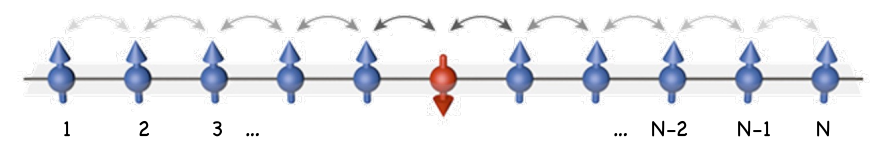
\includegraphics[width=0.7\textwidth]{Immagini/Ising1D_open.png}
    \caption{Esempio di catena di spin per la determinazione della funzione di correlazione fra due spin. Immagine da \cite{galliFSA}.}
    \label{fig: Ising1D_open}
\end{figure}

La funzione di correlazione fra due spin $\sigma_i$ e $\sigma_j$ è definita come

\begin{equation}
    G_{ij}\,=\,\left<\sigma_i \sigma_j\right>\,-\,\left<\sigma_i\right>\left<\sigma_j\right>
    \label{eq: def_corr_fun_Ising1D}
\end{equation}

e consente di valutare se due spin sono correlati o meno. Nel caso del modello di Ising 1D la funzione di correlazione 
risulta essere

\begin{equation}
    G_{i, i+r}\,=\,\left(\tanh{\beta J}\right)^r.
    \label{eq: Ising1D_cor}
\end{equation}

Dall'equazione \eqref{eq: Ising1D_cor} è possibile determinare quale sia la lunghezza di correlazione esprimendo la 
$G_{i, i+r}$ come una funzione esponenzialmente decadente della separazione $r$ fra gli spin in analisi. 

\begin{equation}
    G_{i, i+r}\,=\,e^{r\left[\ln{\left(\tanh{\beta J}\right)}\right]}\,=\,e^{-r/\xi},
    \label{eq: Ising1D_corr_exp}
\end{equation}

da cui risulta che la lunghezza di correlazione è pari a 

\begin{equation}
    \xi\,=\,-\frac{1}{\ln{\left[\tanh{\left(J/k_B T\right)}\right]}}.
    \label{eq: lungh_corr}
\end{equation}

Notiamo che la lunghezza di correlazione è sempre maggiore o uguale a zero. Inoltre, quando la temperatura tende a zero, 
$\xi$ diverge ad infinito. Il fatto che questo accada solamente a temperatura nulla evidenzia come non si abbia correlazione 
(e di conseguenza ordine) a lungo raggio fra gli spin per ogni $T\,\neq\,0$.





\subsection{Simulazioni Monte-Carlo}

L'obiettivo di questa sezione è l'introduzione di delle tecniche Monte-Carlo che consentano di simulare un modello di Ising mono-dimensionale con 
numero di costituenti finito e che presenti condizioni periodiche al contorno, in modo tale che gli spin posti agli estremi della catena 
interagiscano fra loro come primi vicini. Dato che in questo modo tutti gli spin sono equivalenti fra loro ed il sistema è invariante per 
traslazioni, stiamo in pratica simulando un sistema infinito, con un conseguente netto miglioramento della qualità dei risultati. 
Dopo aver definito una condizione iniziale, che solitamente sono quella a temperatura nulla, con tutti gli spin allineati, oppure 
quella a temperatura infinita caratterizzata da momenti magentici orientati casualmente, il primo passo è quello di generare una 
nuova configurazione tentando di invertire uno spin. La differenza in energia fra lo stato di partenza e quello di arrivo determina 
la probabilità d'accettazione della mossa, dato che per l'\textit{algoritmo di Metropolis} \cite{M(RT)2} si ha che 

\begin{equation}
    A\left(\nu\,|\,\mu\right)\,=\,\text{min}\left[1,\,e^{-\beta\left(E_{\nu}\,-\,E_{\mu}\right)}\right]
    \label{eq: Metropolis_1D}
\end{equation}

Chiaramente se la configurazione $\nu$ ha energia inferiore di quella $\mu$, la mossa viene sempre accettata. In caso contrario, è 
possibile che lo spin non venga invertito ed il nuovo elemento della catena di Markov generata dall'algoritmo di Metropolis è identico 
a quello precedente. In seguito è possibile osservare l'implementazione di tale algoritmo in Nim: lo stesso calcolo viene eseguito 
nuovamente ad ogni iterazione, scegliendo lo spin di cui provare il flip in modo casuale.



\subsubsection{Generatore di numeri casuali}

Dato che i metodi Monte-Carlo sono una classe di algoritmi numerici che sfruttano i numeri pseudo-casuali, è auspicabile lavorare 
con un generatore dotato di un lungo periodo (i numeri generati non si ripetono spesso) e che sia efficiente, in modo da ridurre le 
tempistiche computazionali. Le simulazioni che hanno portato ai risultati presenti in questa dispensa sono state effettuate con un 
generatore della famiglia PCG \cite{pcg2014}, di cui è riportata l'implementazione



\begin{minted}[frame=lines, fontsize=\small, bgcolor=blue!10]{nim}
type 
    PCG* = tuple[state, incr: uint64] ##\
    ## The `PCG` type represents the state of a Permuted Congruential 
    ## Generator (PCG), a family of simple fast space-efficient statistically 
    ## good algorithms for random number generation.

    RandomSetUp* = tuple[inState, inSeq: uint64] ##\
    ## The `RandomSetUp` type is used to initialize a `PCG` generator.


proc random*(gen: var PCG): uint64 =
    ## Get a random uint64 from a `PCG`.

    var 
        oldstate = gen.state
        xorshift = uint32(((oldstate shr 18) xor oldstate) shr 27)
        rot = int32(oldstate shr 59)

    gen.state = oldstate * uint64(6364136223846793005) + gen.incr
    result = ((xorshift shr rot) or (xorshift shl ((-rot) and 31)))


proc newRandomSetUp*(rg: var PCG): RandomSetUp {.inline.} = 
    ## Create a new `RandomSetUp` from a `PCG`.
    (rg.random, rg.random)


proc newPCG*(setUp: RandomSetUp): PCG = 
    ## Create a new `PCG` with the given `RandomSetUp`.

    (result.state, result.incr) = (0.uint64, (setUp.inSeq shl 1) or 1)
    discard result.random
    result.state += setUp.inState
    discard result.random


proc rand*(pcg: var PCG): float32 =
    ## Get a random float32 uniformly distributed over the interval (0, 1)
    pcg.random.float32 / 0xffffffff.float32

proc rand*(pcg: var PCG; a, b: float32): float32 =
    ## Get a random float32 uniformly distributed over the interval (a, b)
    a + pcg.rand * (b - a)
\end{minted}    

I numeri pseudo-casuali vengono generati lavorando con interi senza segno, che consentono di fare operazioni fra bit molto efficienti. 
La corretta implementazione è stata testata imponendo un particolare RandomSetUp e valutando la sequenza generata. Sebbene l'implementazione 
del PCG sia riportata nella sezione relativa al modello di Ising mono-dimensionale, tale algoritmo è stato utilizzato anche per l'Ising 2D.



\subsubsection{Termalizzazione}

Una simulazione Monte-Carlo è detta all'equilibrio nel momento in cui viene correttamente campionato il peso statistico di Boltzmann 
$p\left(\mu\right)$. Se il sistema viene inizializzato in uno dei due stati presentati in precedenza, ossia quello a temperatura 
nulla (con spin paralleli) oppure a $T$ infinita (con spin orientati casualmente up oppure down) e si vuole performare una simulazione a 
temperatura finita, sarà necessario del tempo computazionale prima che venga raggiunto l'equilibrio, poichè sara necessario accettare 
alcune mosse.

Un modo qualitativo per valutare la durata della termalizzazione consiste nel graficare una quantità d'interesse, 
come può essere la magnetizzazione oppure l'energia interna del sistema. Tali osservabili presenteranno una fase di transitorio 
iniziale in cui il sistema si scorrela dalla condizione iniziale, per poi fluttuare attorno ad un valore pressochè costante. Non è 
sempre garantito che si raggiunga l'equilibrio, in quanto è possibile rimanere bloccati in uno stato metastabile per tempistiche 
computazionali relativamente lunghe. Per evitare di valutare in maniera errata la durata della fase di termalizzazione è consigliabile 
eseguire lo stesso processo per diverse condizioni iniziali e per diversi seed del generatore di numeri casuali, in modo da considerare 
diverse traiettorie nello spazio delle fasi.  




\subsubsection{Misure e Data-Blocking}

Una volta che il sistema ha raggiunto l'equilibrio, è possibile misurare le osservabili d'interesse senza che i valori d'aspettazione 
siano influenzati dalla fase di transitorio. Per valutare la durata minima della simulazione che consenta di ottenere delle stime 
statisticamente significative è necessaria una misura del tempo di correlazione $t_c$, che esplicita quale sia il numero di mosse 
da effettuare per passare fa uno stato ad un secondo significativamente differente da quello di partenza. Il modo migliore per 
calcolare $t_c$ consiste nello sfruttare la funzione di autocorrelazione temporale, definita per la magnetizzazione come 

\begin{equation}
    \chi\left(t\right)\,=\,\frac{\left<m\left(t'\right)m\left(t'\,+\,t\right)\right>_{t'}\,-\,\left<m\right>^2}{\sigma^2_m}
    \label{eq: auto_corr_m}
\end{equation}

L'autocorrelazione solitamente presenta una caduta esponenziale con tempo caratteristico pari a quello di correlazione

\begin{equation}
    \chi\left(t\right)\,\sim\,e^{-t/t_c}.
    \label{eq: auto_corr_cad_exp}
\end{equation}

Se si considerano due campioni presi ad un $t_c$ di distanza, la funzione di autocorrelazione assume in presenza di un tale 
intervallo temporale un valore di $1/e$, ancora particolarmente significativo. Se si vuole lavorare con quantità realmente indipendenti 
è necessario campionare a $t\,>\,t_c$; solitamente si impone $t\,=\,t_c$ in modo che il numero di misure significative in una 
simulazione di durata $t_{max}$ è pari a 

\begin{equation}
    n\,=\,\frac{t_{max}}{2 t_c}.
    \label{eq: num_ind_samp}
\end{equation}

Per evitare bias nel campionamento e per ottenere dei valori d'aspettazione adeguati è possibile utilizzare la tecnica del 
data-blocking. Le misure delle osservabili di interesse effettuate durante la simulazione, a distanze temporali del tempo di correlazione, 
vengono divise in gruppi, per ciascuno dei quali viene calcolato il valor medio. La dispersione di questi valori medi fornisce una 
stima dell'errore associato alla grandezza calcolata. In Figura \ref{fig: data_block_tech} è presentata visivamente la tecnica del data-
blocking. Le quantità $g_i$ sono le medie di ciascun gruppo.

\begin{figure}[H]
    \centering
    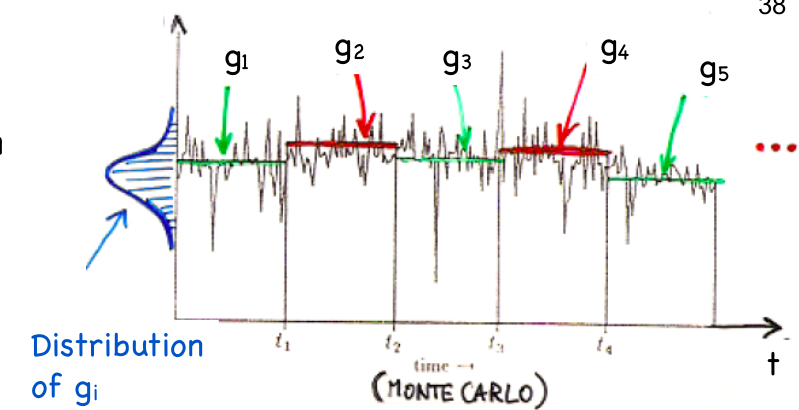
\includegraphics[width=0.6\textwidth]{Immagini/data_blocking.png}
    \caption{Esempio di applicazione della tecnica del data-blocking. Immagine da \cite{galliLSN}.}
    \label{fig: data_block_tech}
\end{figure}

Per determinare quale sia la lunghezza dei blocchi tale da garantire che le medie siano statisticamente indipendenti, si può 
sfruttare il teorema del limite centrale. Nel momento in cui si aumenta la lunghezza dei blocchi, l'errore calcolabile come 

\begin{equation}
    \sigma_{\left<g\right>}\,=\,\sqrt{\frac{1}{N-1}\left(\left<g^2\right>\,-\,\left<g\right>^2\right)}
    \label{eq: error_data_block}
\end{equation}

tende a quello puramente statistico (poichè si va a perdere la correlazione fra le stime) e dopo una certa lunghezza $L$ dei blocchi 
non aumenta più, ma satura ad un valore costante. La lunghezza di saturazione è la minima accettabile per produrre delle stime adeguate. 
Chiaramente maggiore è il numero di blocchi (ossia più lunga è la simulazione), migliore sarà la stima finale della osservabile 
d'interesse.





\subsection{Simulazioni}

La prima fase della simulazione del modello di Ising 1D è incentrata sulla determinazione dei parametri ottimali per ottenere 
dei valori d'aspettazione statisticamente rilevanti, in modo tale da poter effettuare il confronto con il valor vero noto in letteratura. In 
questa fase preliminare ho lavorato con le seguenti quattro lunghezze del modello di Ising 1D e le seguenti quattro temperature 

\begin{equation}
    l\,\in\,\left\{1000,\,3000,\,6000,\,10000\right\}
    \label{eq: dim_sim_Ising1D}
\end{equation}

\begin{equation}
    T\,\in\,\left\{0.5,\,1.0,\,1.5,\,2.0\right\}
    \label{eq: temp_sim_Ising1D}
\end{equation}

Per ognuna di queste coppie dimensione-temperatura ho considerato quattro seed differenti del generatore di numeri casuali in modo da 
poter analizzare il comportamento del sistema lungo differenti traiettorie nello spazio delle fasi. 



\subsubsection{Termalizzazione}

La lunghezza della fase di termalizzazione dipende fortemente dal valore della temperatura a cui viene svolta la simulazione, come è 
possibile osservare nelle seguenti Figure in cui sono riportati i risultati ottenuti raggruppati per lunghezza della catena di spin. 
La durata maggiore della termalizzazione si ha per la temperatura inferiore, ossia $T\,=\,0.5$, poichè per giungere ad una configurazione 
ordinata (come evidente dal valore della magnetizzazione tendente ad uno) è necessario un tempo computazionale maggiore legato alla 
necessità di orientare tutti gli spin in modo concorde.

\newpage

\vspace*{\fill}

\begin{figure}[htbp]
    \centering
    \begin{minipage}{0.45\textwidth}  
      \centering
      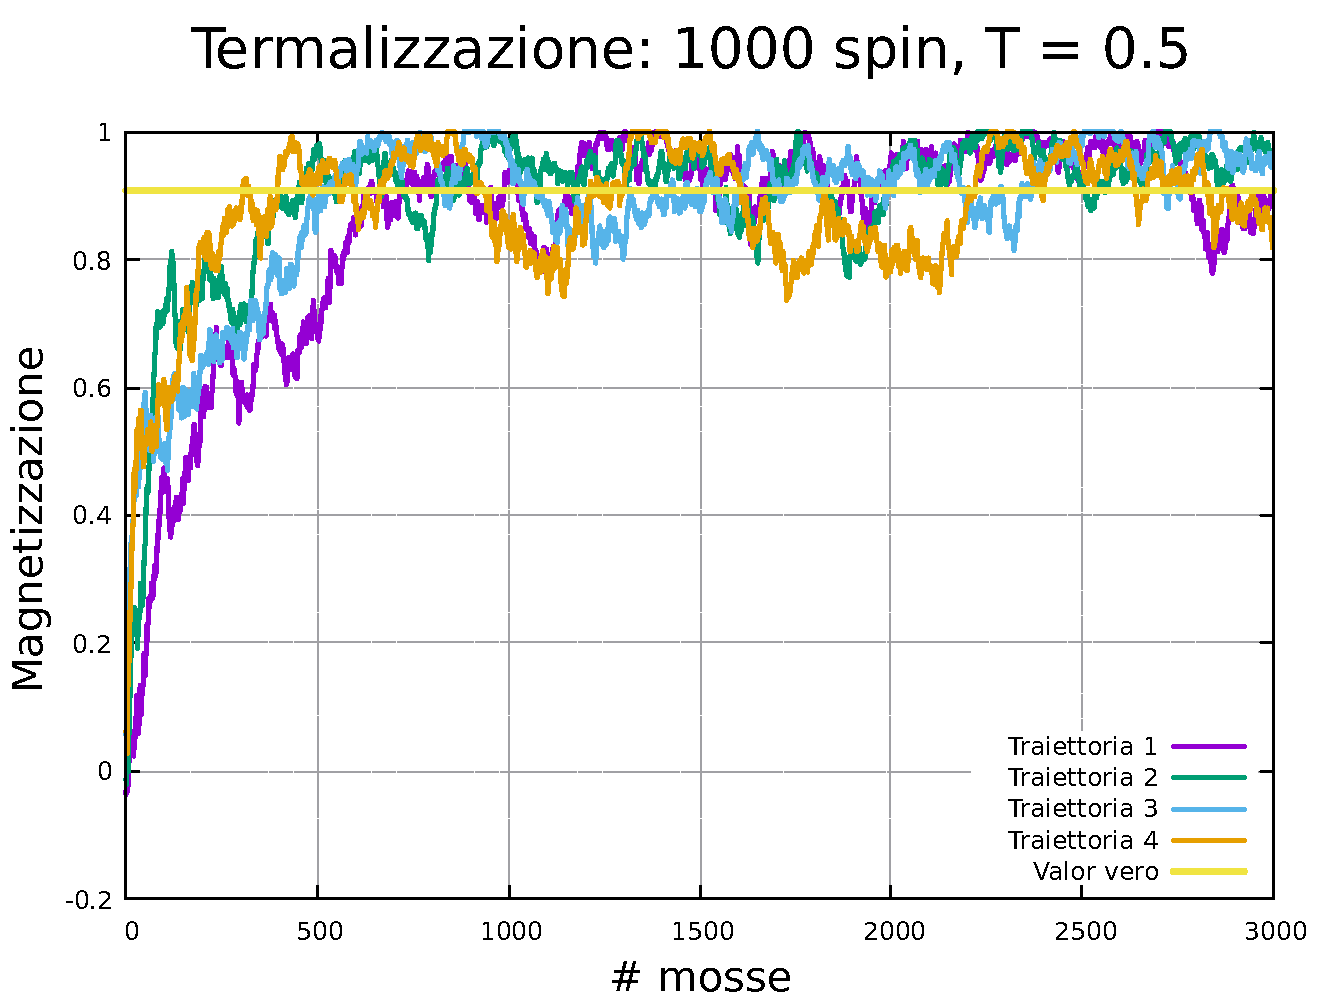
\includegraphics[page=1, width=\textwidth]{Immagini/simIsing1D/term/term_1000_0.5.pdf}
      \caption{$T\,=\,0.5$}
    \end{minipage}\hfill
    \begin{minipage}{0.45\textwidth}  
      \centering
      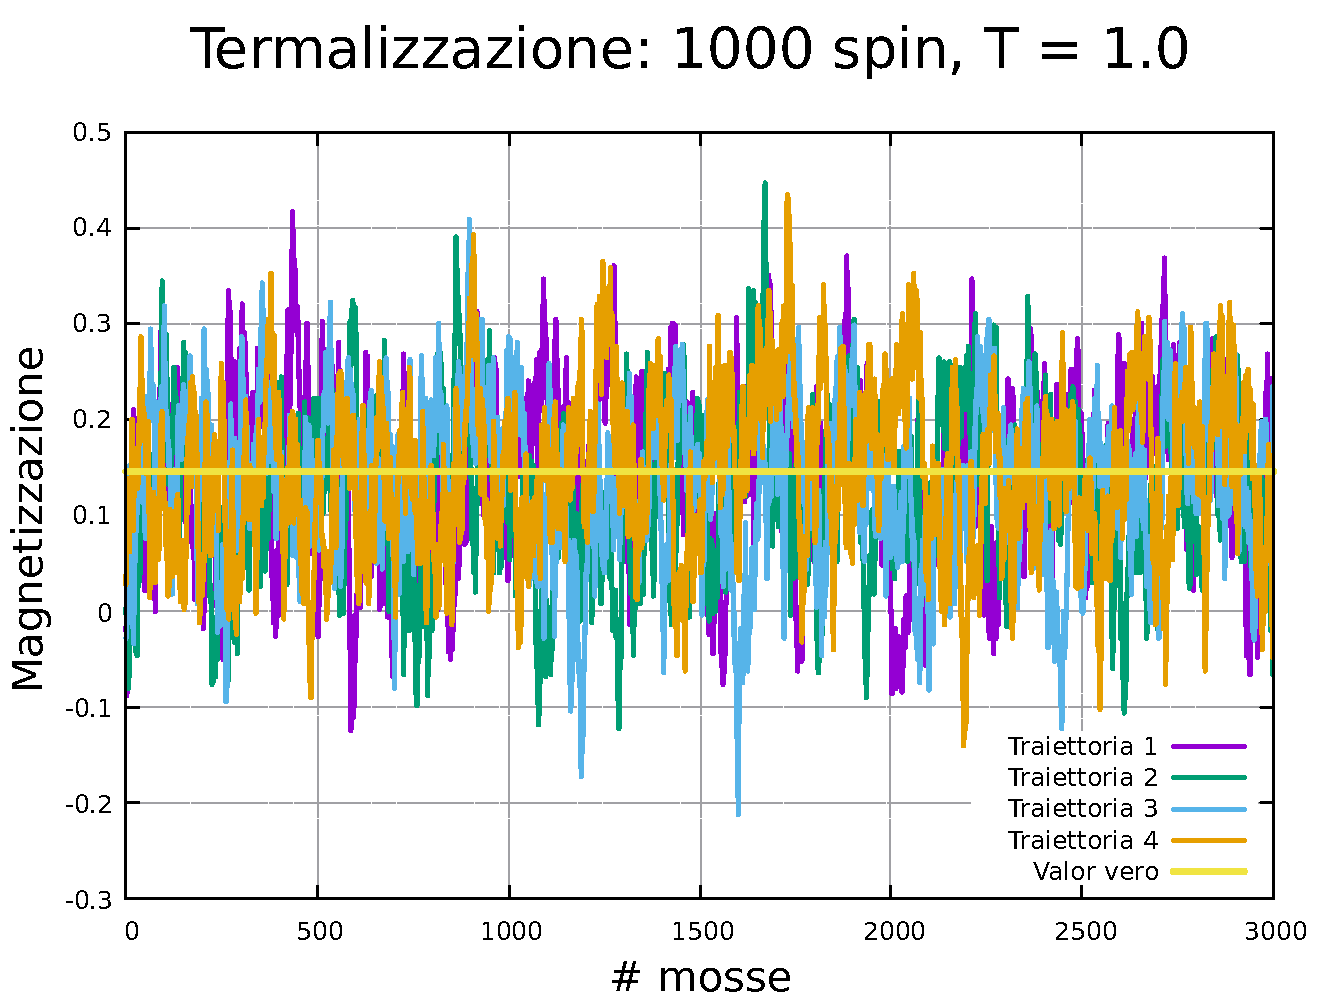
\includegraphics[page=1, width=\textwidth]{Immagini/simIsing1D/term/term_1000_1.0.pdf}
      \caption{$T\,=\,1.0$}
    \end{minipage}
    \vskip\baselineskip 
  
    \begin{minipage}{0.45\textwidth}  
      \centering
      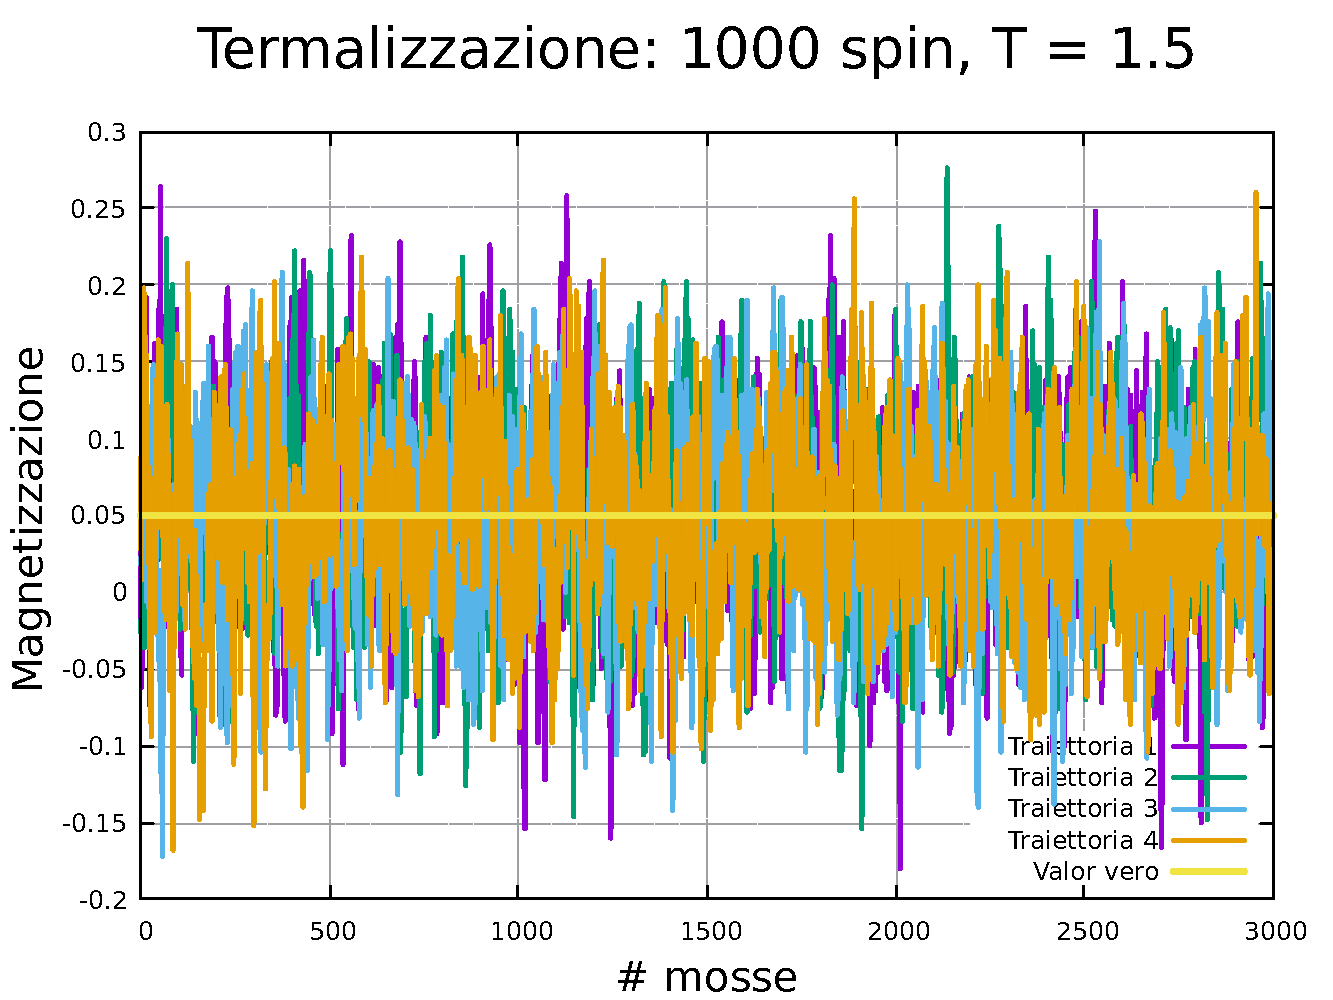
\includegraphics[page=1, width=\textwidth]{Immagini/simIsing1D/term/term_1000_1.5.pdf}
      \caption{$T\,=\,1.5$}
    \end{minipage}\hfill
    \begin{minipage}{0.45\textwidth}  
      \centering
      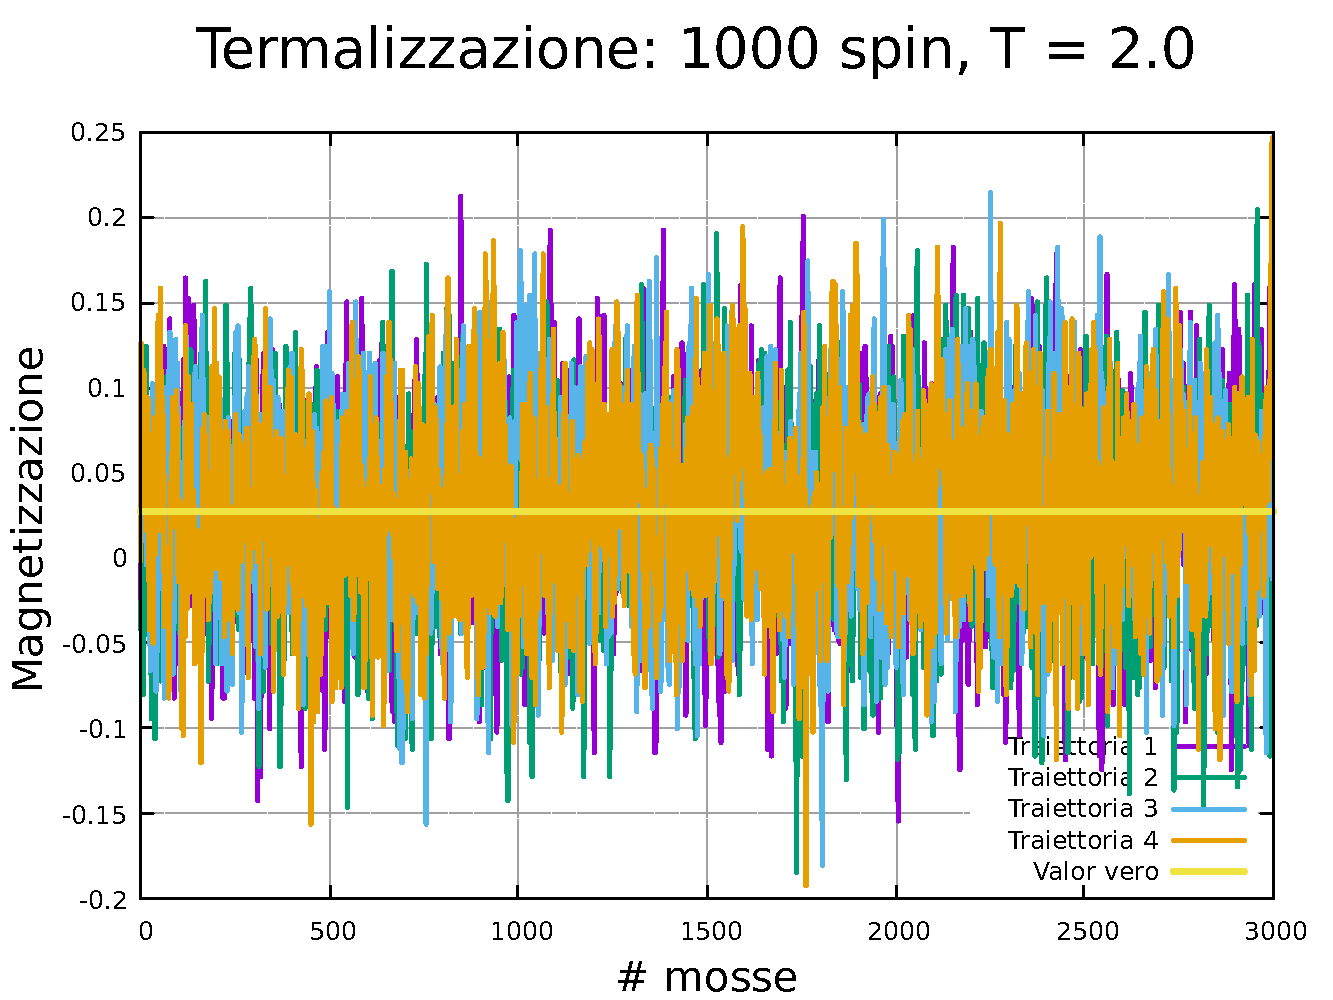
\includegraphics[page=1, width=\textwidth]{Immagini/simIsing1D/term/term_1000_2.0.pdf}
      \caption{$T\,=\,2.0$}
    \end{minipage}
    \caption{Studio della termalizzazione di un modello di Ising 1D costituito da 1000 spin.}
\end{figure}

\vspace*{\fill}

\newpage

\vspace*{\fill}

\begin{figure}[htbp]
    \centering
    \begin{minipage}{0.45\textwidth}  
      \centering
      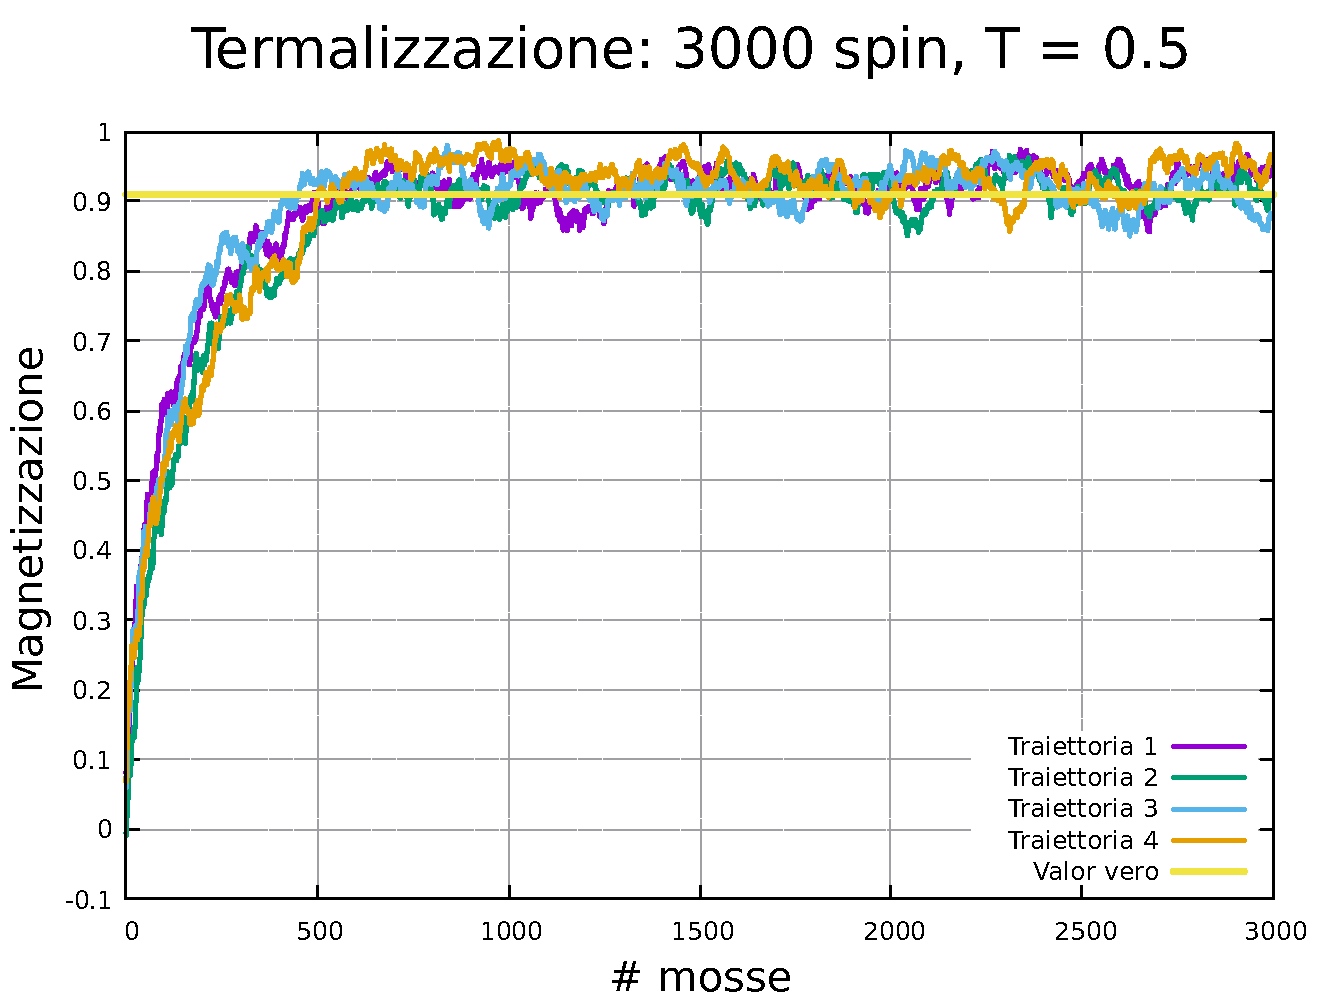
\includegraphics[page=1, width=\textwidth]{Immagini/simIsing1D/term/term_3000_0.5.pdf}
      \caption{$T\,=\,0.5$}
    \end{minipage}\hfill
    \begin{minipage}{0.45\textwidth}  
      \centering
      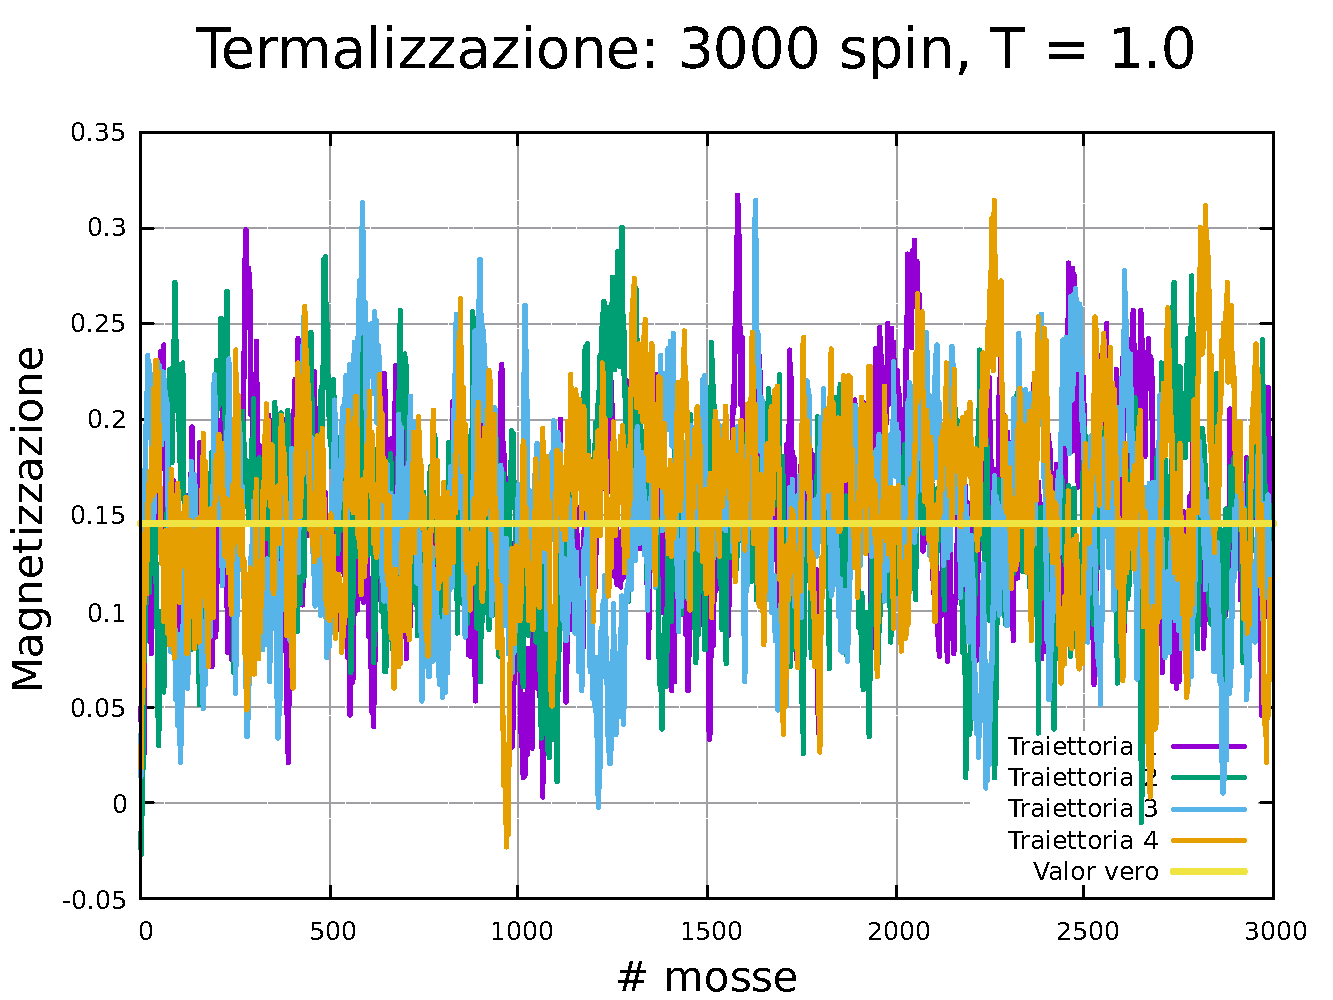
\includegraphics[page=1, width=\textwidth]{Immagini/simIsing1D/term/term_3000_1.0.pdf}
      \caption{$T\,=\,1.0$}
    \end{minipage}
    \vskip\baselineskip 
  
    \begin{minipage}{0.45\textwidth}  
      \centering
      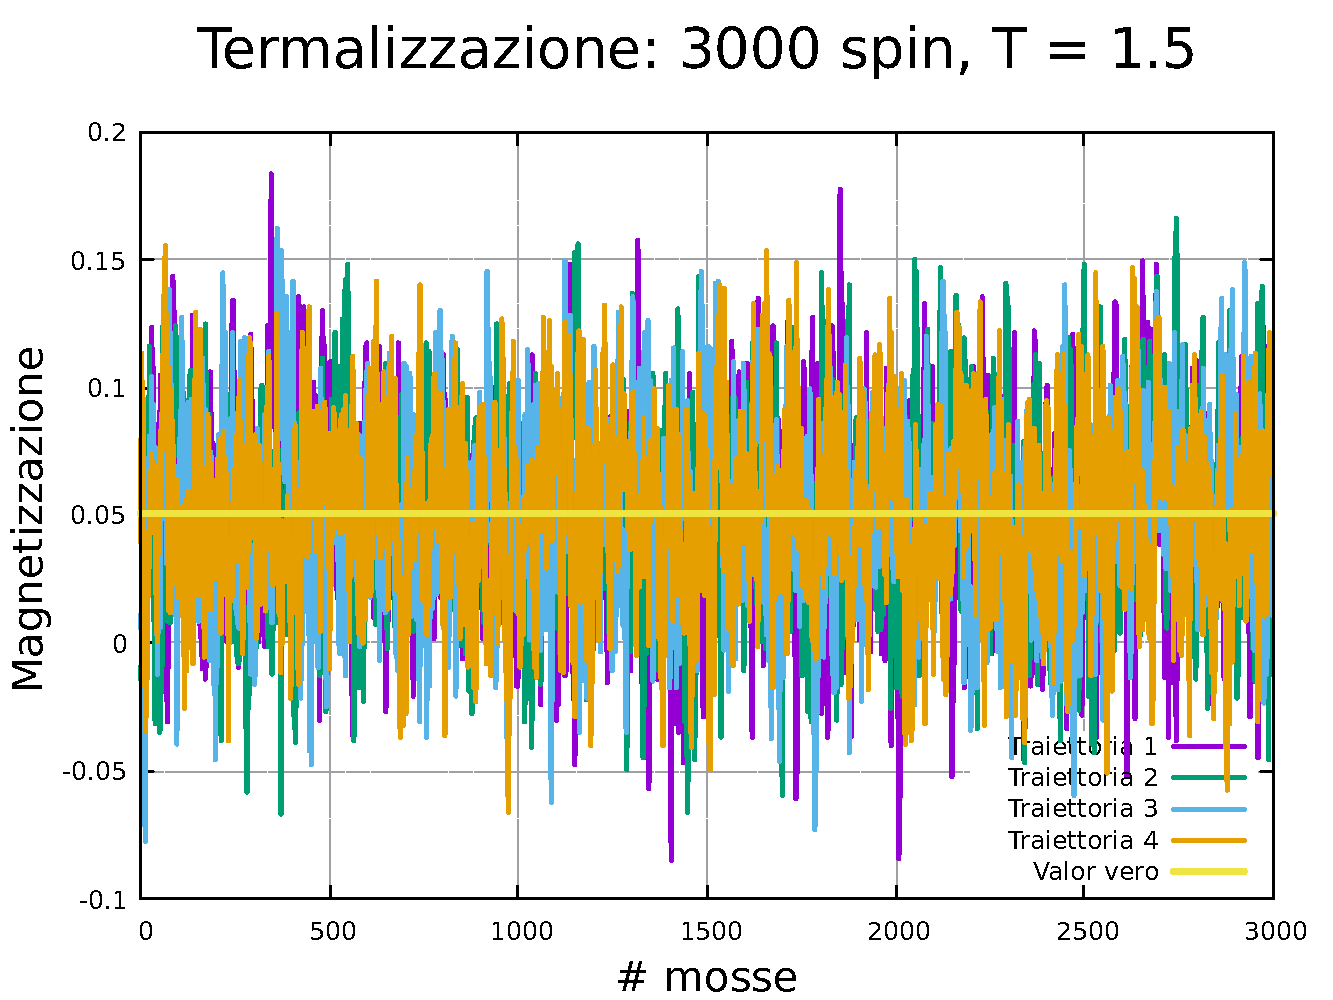
\includegraphics[page=1, width=\textwidth]{Immagini/simIsing1D/term/term_3000_1.5.pdf}
      \caption{$T\,=\,1.5$}
    \end{minipage}\hfill
    \begin{minipage}{0.45\textwidth}  
      \centering
      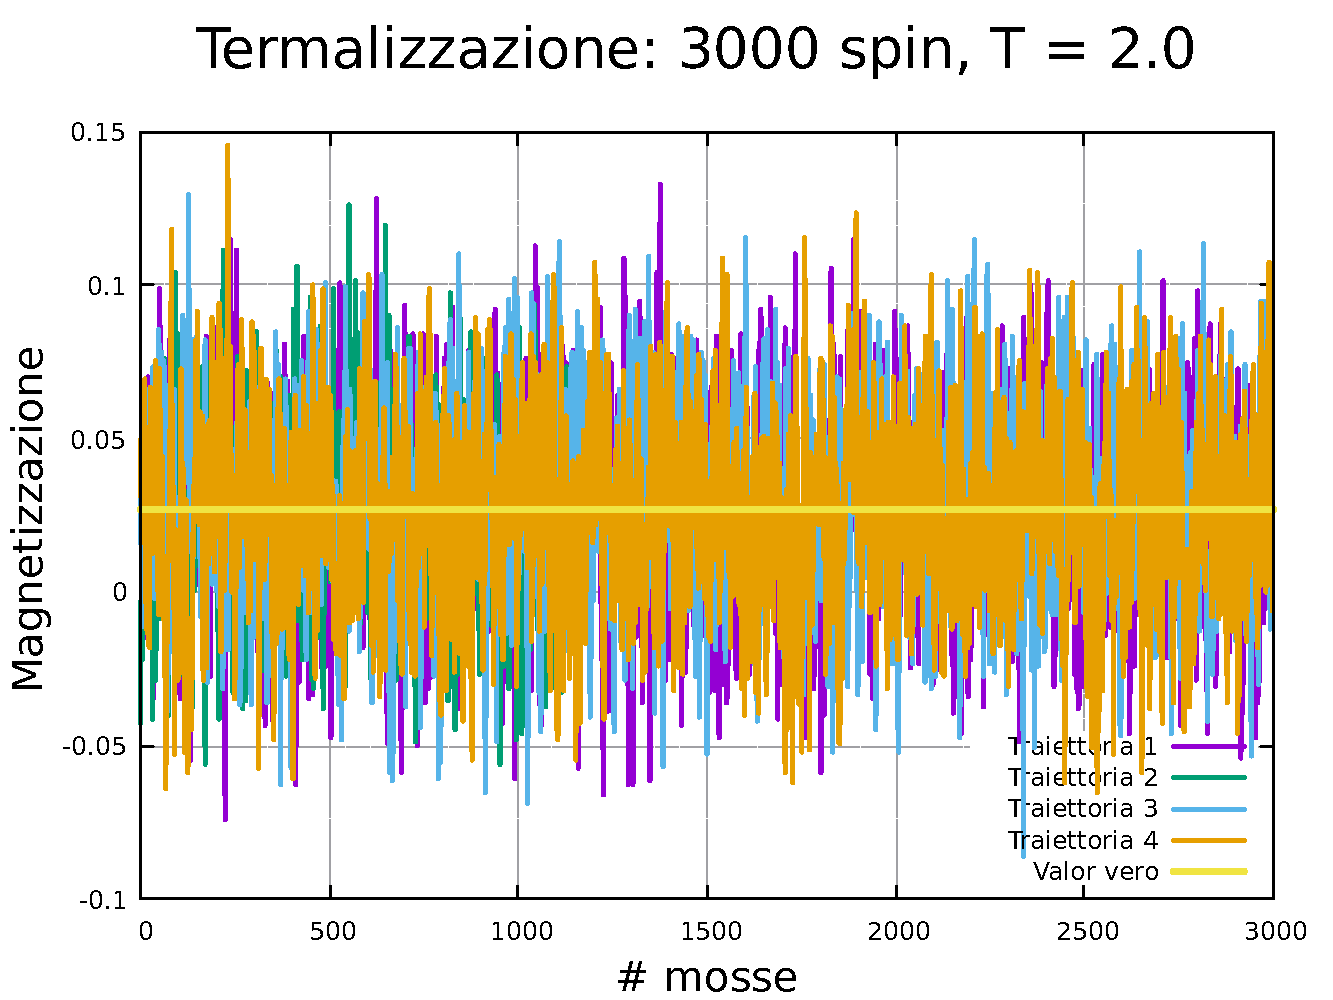
\includegraphics[page=1, width=\textwidth]{Immagini/simIsing1D/term/term_3000_2.0.pdf}
      \caption{$T\,=\,2.0$}
    \end{minipage}
    \caption{Studio della termalizzazione di un modello di Ising 1D costituito da 3000 spin.}
\end{figure}

\vspace*{\fill}

\newpage

\vspace*{\fill}

\begin{figure}[htbp]
    \centering
    \begin{minipage}{0.45\textwidth}  
      \centering
      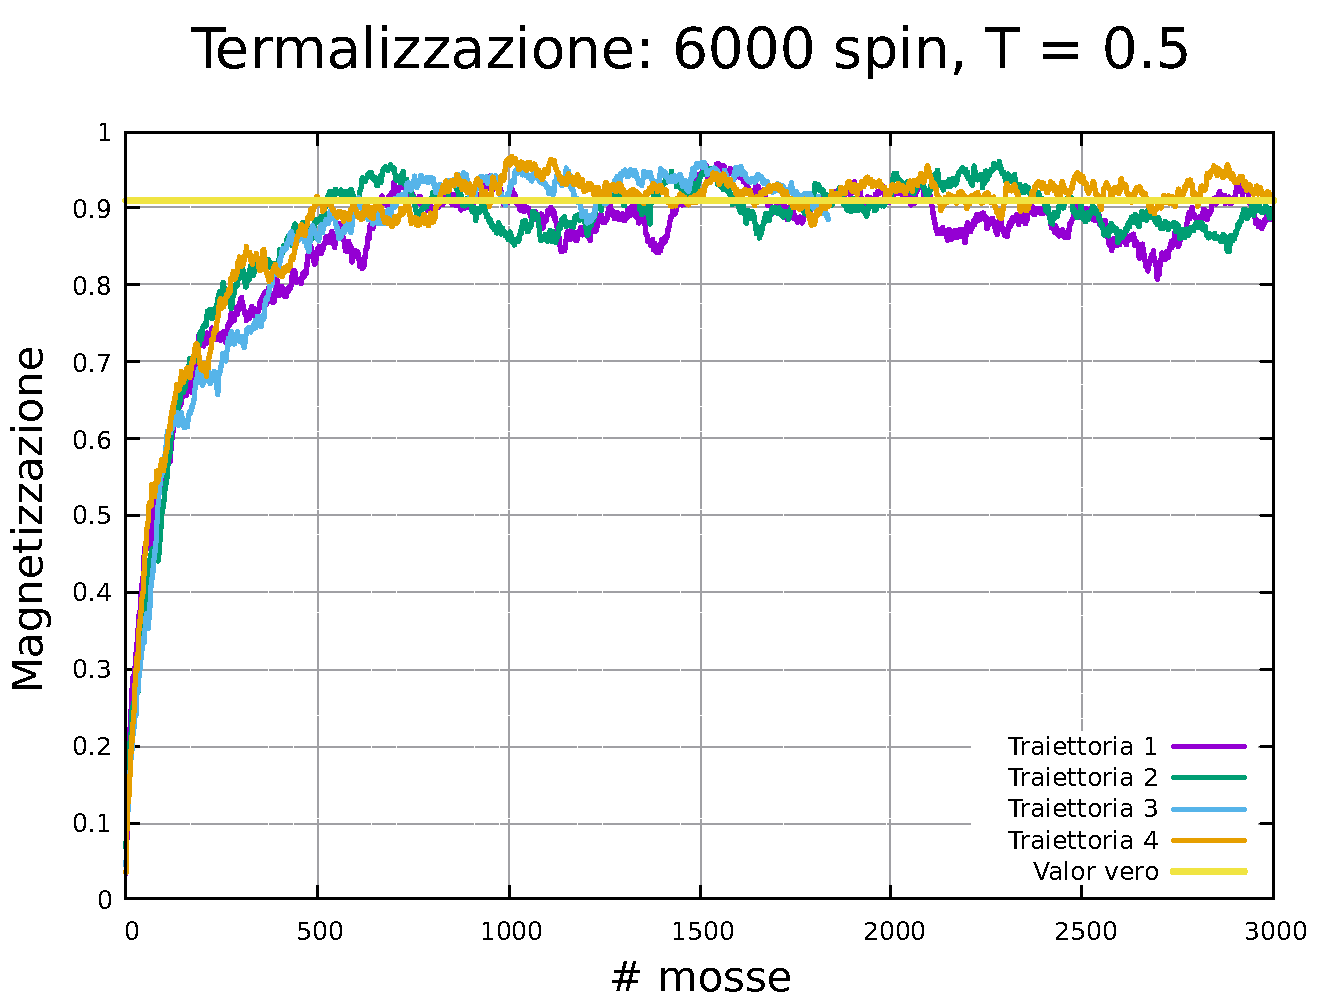
\includegraphics[page=1, width=\textwidth]{Immagini/simIsing1D/term/term_6000_0.5.pdf}
      \caption{$T\,=\,0.5$}
    \end{minipage}\hfill
    \begin{minipage}{0.45\textwidth}  
      \centering
      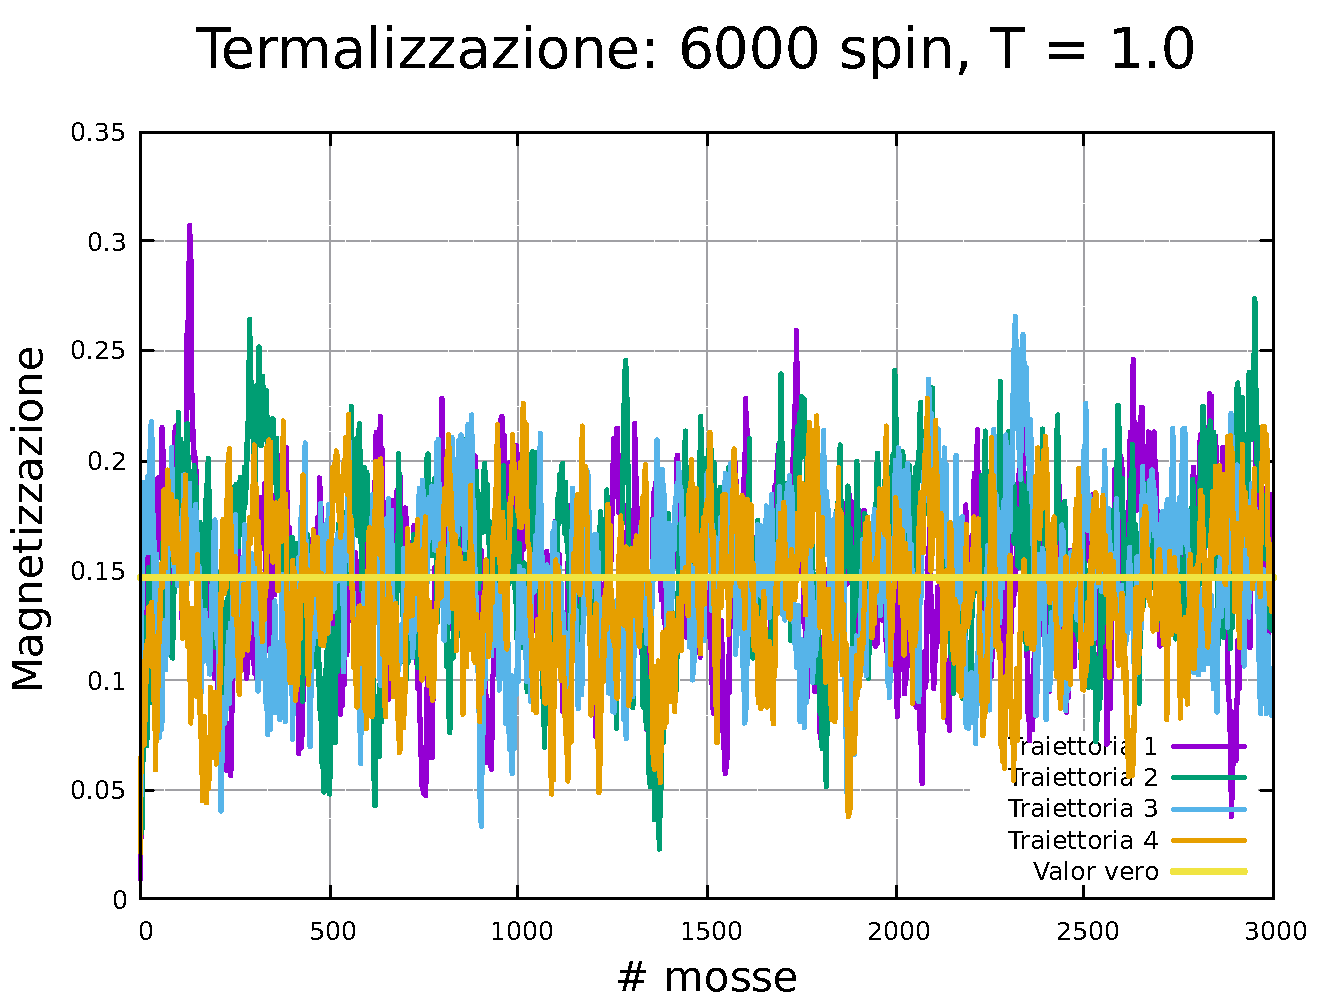
\includegraphics[page=1, width=\textwidth]{Immagini/simIsing1D/term/term_6000_1.0.pdf}
      \caption{$T\,=\,1.0$}
    \end{minipage}
    \vskip\baselineskip 
  
    \begin{minipage}{0.45\textwidth}  
      \centering
      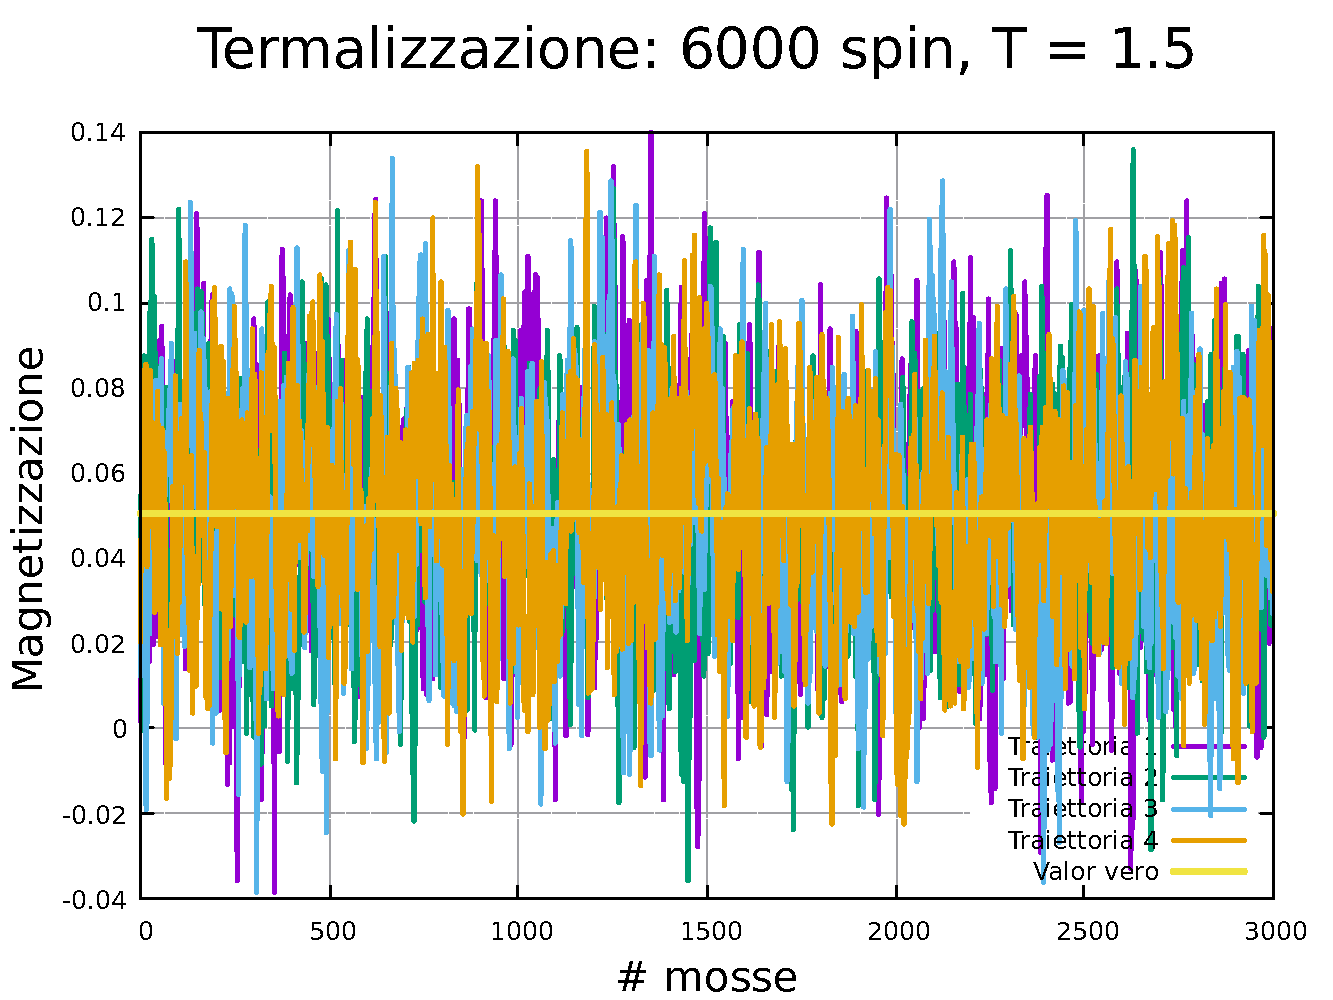
\includegraphics[page=1, width=\textwidth]{Immagini/simIsing1D/term/term_6000_1.5.pdf}
      \caption{$T\,=\,1.5$}
    \end{minipage}\hfill
    \begin{minipage}{0.45\textwidth}  
      \centering
      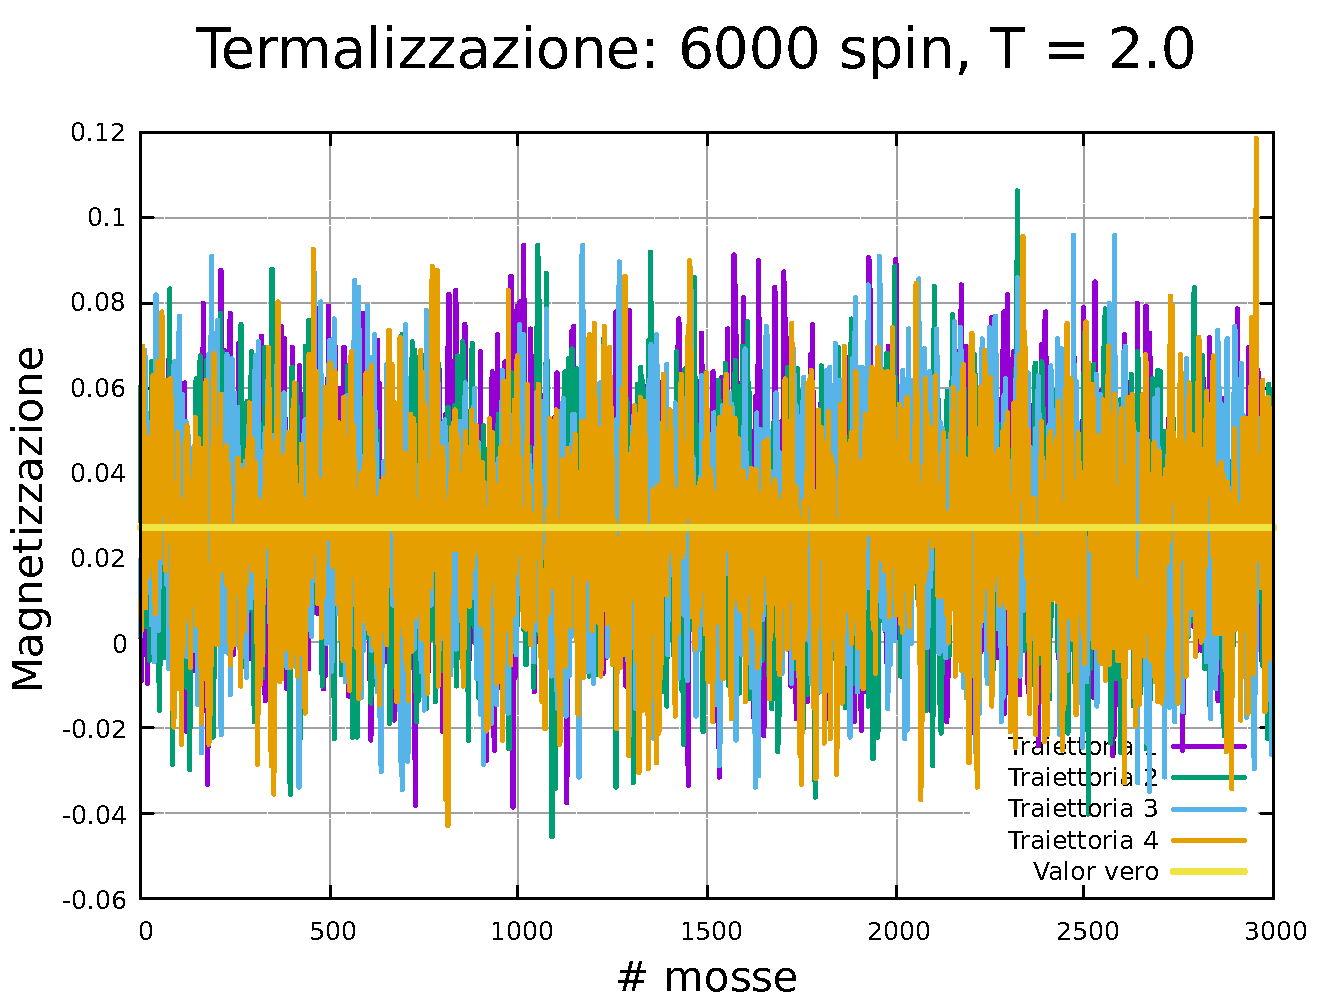
\includegraphics[page=1, width=\textwidth]{Immagini/simIsing1D/term/term_6000_2.0.pdf}
      \caption{$T\,=\,2.0$}
    \end{minipage}
    \caption{Studio della termalizzazione di un modello di Ising 1D costituito da 6000 spin.}
\end{figure}

\vspace*{\fill}

\newpage

\vspace*{\fill}

\begin{figure}[htbp]
    \centering
    \begin{minipage}{0.45\textwidth}  
      \centering
      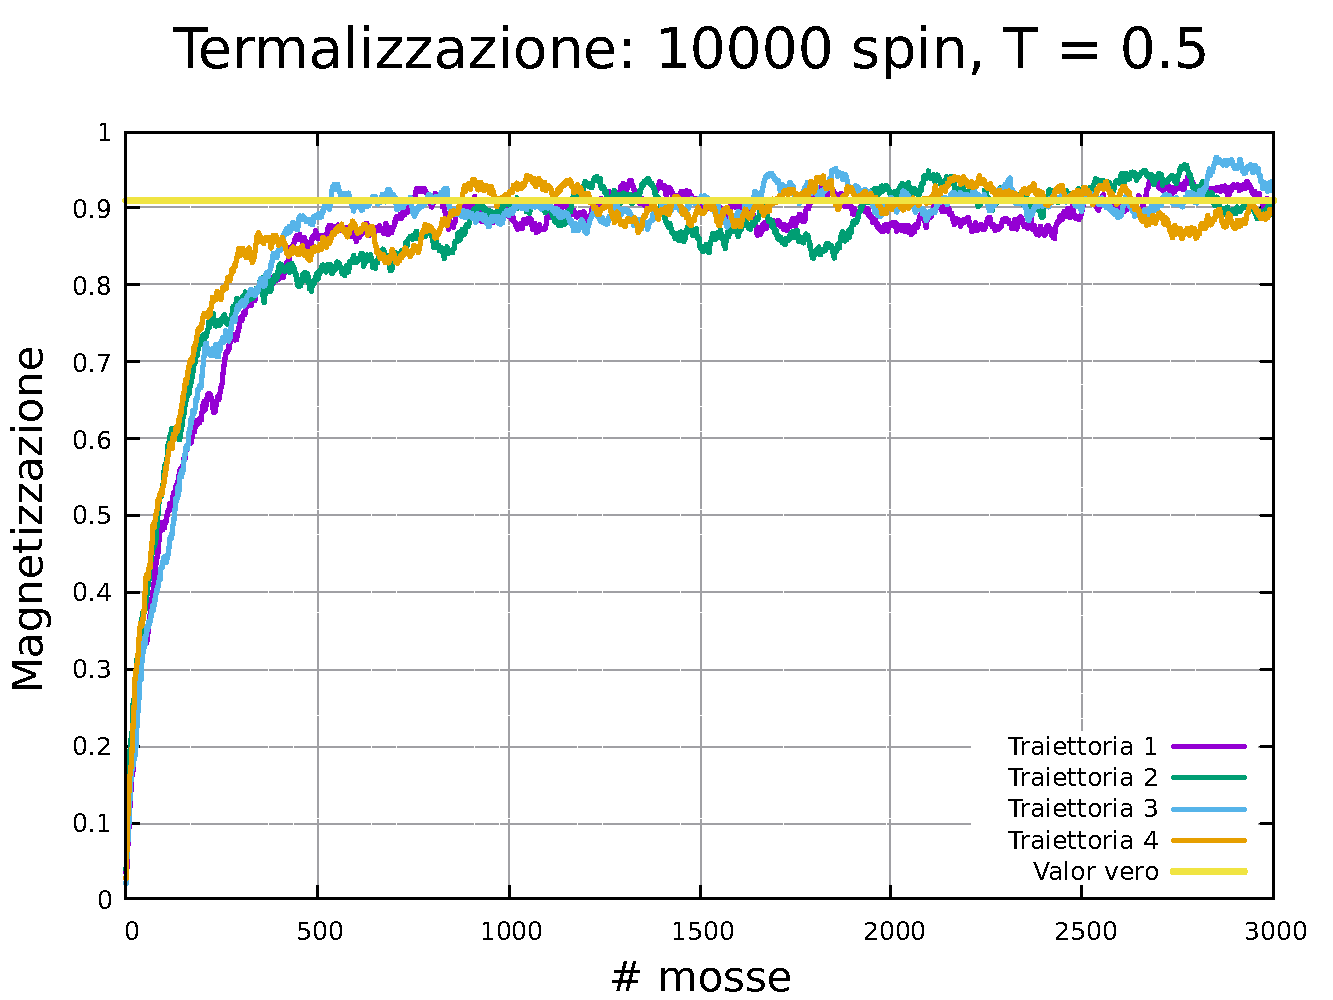
\includegraphics[page=1, width=\textwidth]{Immagini/simIsing1D/term/term_10000_0.5.pdf}
      \caption{$T\,=\,0.5$}
    \end{minipage}\hfill
    \begin{minipage}{0.45\textwidth}  
      \centering
      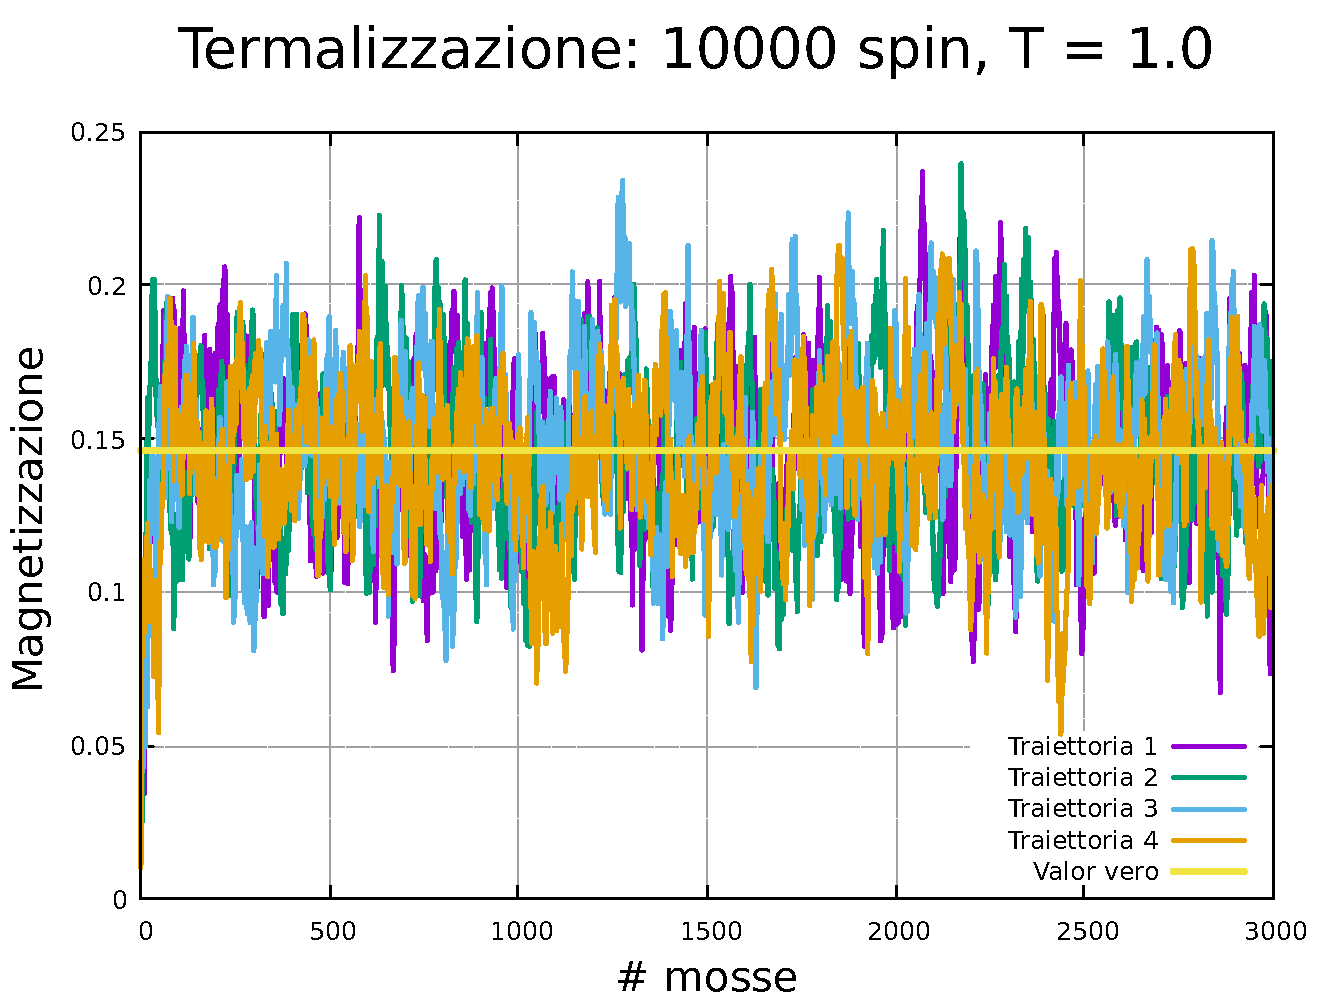
\includegraphics[page=1, width=\textwidth]{Immagini/simIsing1D/term/term_10000_1.0.pdf}
      \caption{$T\,=\,1.0$}
    \end{minipage}
    \vskip\baselineskip 
  
    \begin{minipage}{0.45\textwidth}  
      \centering
      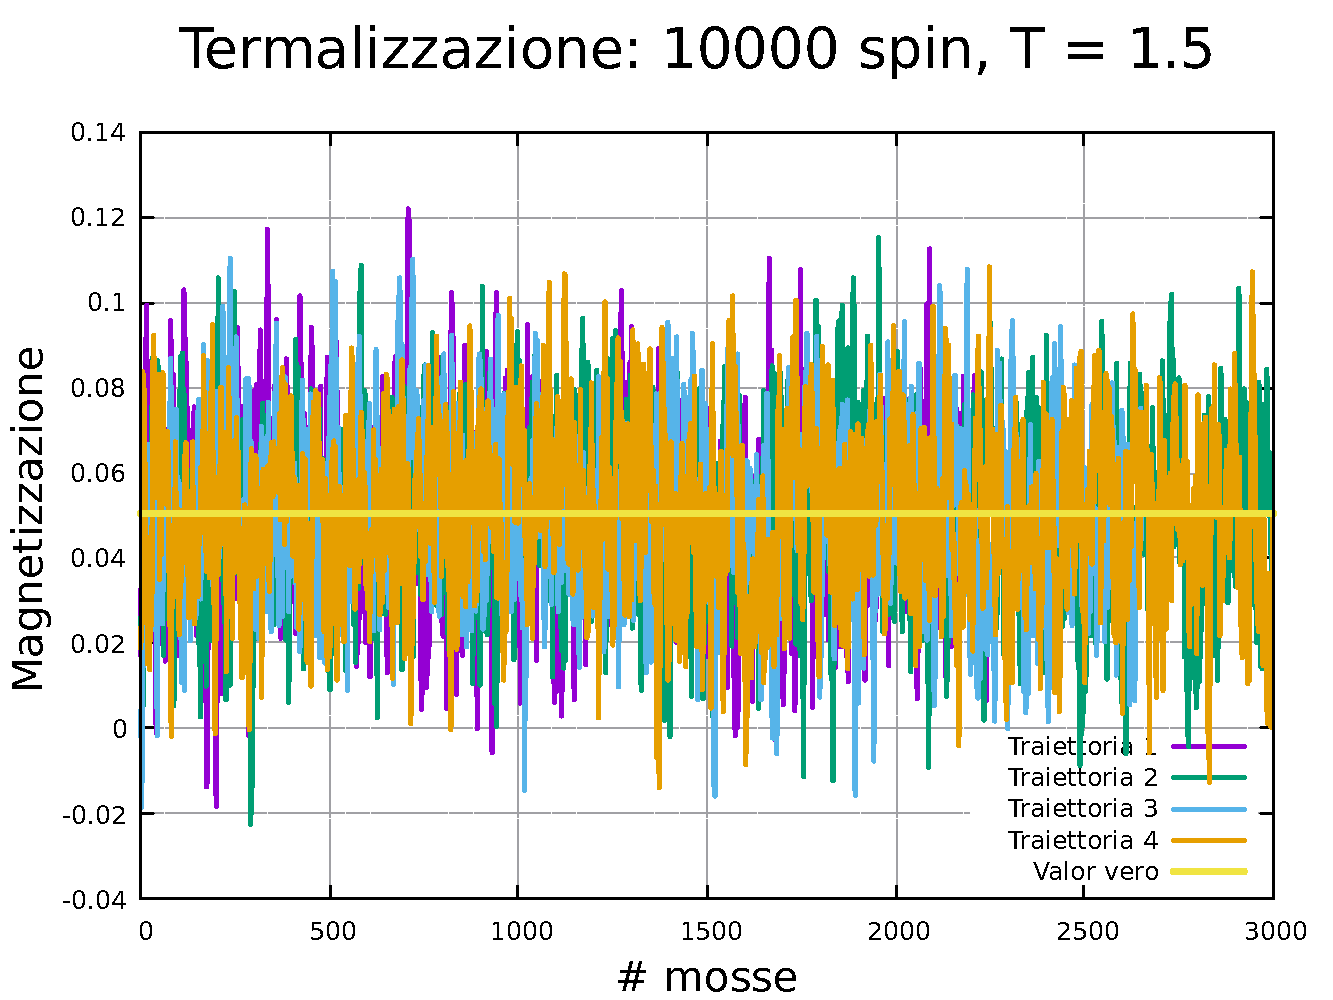
\includegraphics[page=1, width=\textwidth]{Immagini/simIsing1D/term/term_10000_1.5.pdf}
      \caption{$T\,=\,1.5$}
    \end{minipage}\hfill
    \begin{minipage}{0.45\textwidth}  
      \centering
      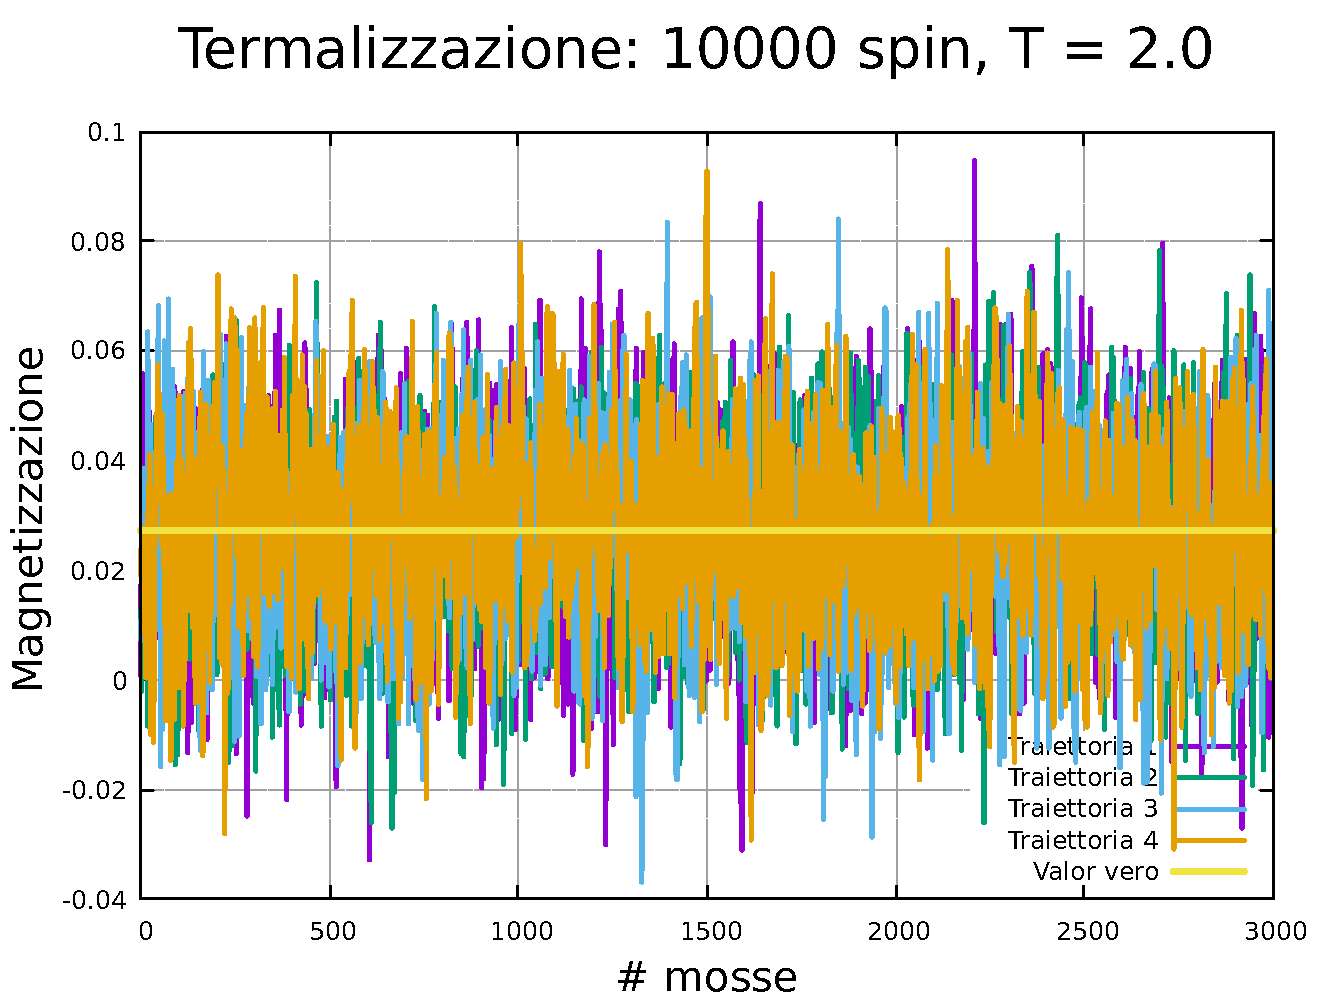
\includegraphics[page=1, width=\textwidth]{Immagini/simIsing1D/term/term_10000_2.0.pdf}
      \caption{$T\,=\,2.0$}
    \end{minipage}
    \caption{Studio della termalizzazione di un modello di Ising 1D costituito da 10000 spin.}
\end{figure}

\vspace*{\fill}

\newpage